\chapter{Study of Literature}

\textbf{Author: } 

\section{Different Approaches to the Problem}

\section{Depth perception}
[TODO: humans, two eyes - gleich wie bei unserem Aufbau]

\subsection{Depth sensation}
[TODO: Pigeons, deer, children (visual cliff)]

\section{Stereo Camera}
The challenge of sensing distances to various objects has been solved using stereo vision cameras. Computer stereo vision systems use two horizontally displaced cameras to take two images which then are both processed together to gather the information on the depth of the images. This process can be rather complicated as the distortions (more specifically the barrel distortion and the tangential distortion) of the images have to be undone, before the two images are projected onto a common plane, a disparity map can be created by comparison of the two images and a 3d point cloud can be generated from it. In most robotics applications this point cloud is then filtered in search of some object, which distance was sought-after.

\subsection{Distortion}
Barrel distortion occurs when the lens used by the camera has a higher magnification at the centre of the image than at the sides. This distortion can be visualized as seen in Figure~\ref{pic:methodology_stereoCamera_distortion_barrelDistortion}.

\begin{figure}[h!]
	\centering
	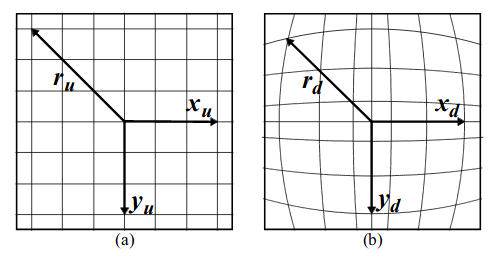
\includegraphics[width=4.5in]{img/methodology_stereoCamera_distortion_barrelDistortion.png}
	\caption{The left shows the original image composed of straight horizontal and vertical lines. On the right image the effect of the barrel distortion can be perceived, which causes the lines to curve toward the outside of the image, causing the lines to appear in a barrel like shape.[TODO: change image to own]}
	\label{pic:methodology_stereoCamera_distortion_barrelDistortion}
\end{figure}

To undo this distortion the pixel values in an undistorted image have to be calculated based on the pixel values in the distorted image.

\begin{equation}
r_u = r_d(1+k r_d^2)
\end{equation}

describes the calculation which computes the distance from the centre in the undistorted image ($r_u$) based on the distance from the centre in the distorted image ($r_d$) and some distortion parameter $k$, which is specific to the lens used. Gribbon et.al. note in their work \footcite{Gribbon_Barrel_Distortion_Correction_Algorithm} that this rarely is an integer value, therefore different equations are proposed:

\begin{equation}
x_d = x_u M(k,r_u^2) \hspace{30pt} y_d = y_u M(k, r_u^2)
\end{equation}

where the magnification factor $M(k,r_u^2)$ is

\begin{equation}
M(k,r_u^2) = \frac{1}{1+k * M(k,r_u^2)^2 * r_u^2}
\end{equation}

Tangential distortion in comparison to barrel distortion displaces points along the tangent of a circle placed at the centre of the image as seen in Figure~\ref{pic:methodology_stereoCamera_distortion_tangentialDistortion}.

\begin{figure}[h!]
	\centering
	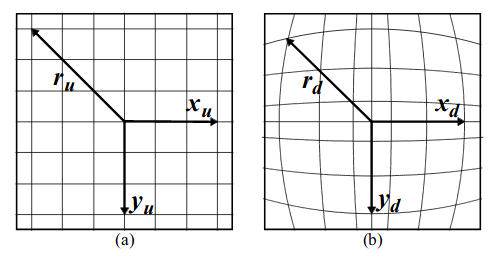
\includegraphics[width=2in]{img/methodology_stereoCamera_distortion_tangentialDistortion.png}
	\caption{A point $P$ is distorted along the tangent $t$ of a circle placed at the middle of the image $C$ with a radius $r$ to a point $P'$. Distortions of this form are called tangential distortions.}
	\label{pic:methodology_stereoCamera_distortion_tangentialDistortion}
\end{figure}

The radius of the circle in Figure~\ref{pic:methodology_stereoCamera_distortion_tangentialDistortion} is dependent on the point $P$. It can be calculated as the length between $P$ and $C$. The length of the vector $PP'$ is not uniform for all points and therefore depends on point $P$.

\subsection{Image Rectification}
Image Rectification projects multiple images taken from different points of view onto a common plane. 

\begin{figure}[h!]
	\centering
	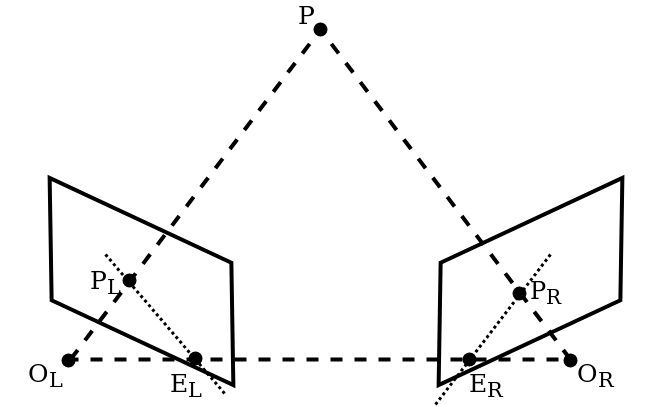
\includegraphics[width=4in]{img/methodology_stereoCamera_imageRectification.png}
	\caption{Two images containing some point $P$ are taken from the two points $O_L$ and $O_R$. Point $P$ is projected in the image planes as points $P_L$ and $P_R$. $E_L$ and $E_R$ depict the epipoles.}
	\label{pic:methodology_stereoCamera_imageRectification}
\end{figure}

Chan et. al. propose an image rectification algorithm \footcite{Chen_New_Image_Rectification_Algorithm}, which follows this sequence of events:

\begin{enumerate}
	\item At least seven matching points visible on both images are found.
	\item The fundamental matrix (as well as the epipoles) are estimated.
	\item The common region is identified (using epipolar geometry constraints).
	\item The epipolar line is transferred and the Bresenham algorithm\footcite{Bresenham_Linear_Algorithm_For_Incremental_Digital_Display_Of_Circular_Arcs} is used to extract pixel values.
	\item The rectified image is resampled.
\end{enumerate}

\subsection{Disparity Map}

\subsection{3d point cloud}


[Input: Paper (gleiches Problem ohne NN) finden - Peter]

[Input: Video (eine Kamera, Entfernung zu Punkt (größe bekannt)) finden (ohne NN) - Peter]


[Vielleicht ist irgendetwas davon spannend:
Links im Tex file
%https://ieeexplore.ieee.org/abstract/document/6399589
%https://ieeexplore.ieee.org/abstract/document/100062
%https://ieeexplore.ieee.org/abstract/document/6079296
%https://www.sciencedirect.com/science/article/pii/S0957417414008161
%http://neuralnetworksanddeeplearning.com/chap1.html
%https://patents.google.com/patent/US8164628B2/en
%https://apps.dtic.mil/docs/citations/ADA366182
%https://ieeexplore.ieee.org/abstract/document/1087003
%https://digital-library.theiet.org/content/conferences/10.1049/cp.2010.0495
%https://www.isca-speech.org/archive/interspeech_2010/i10_1045.html
%https://ieeexplore.ieee.org/abstract/document/6639344
%https://www.sciencedirect.com/science/article/pii/B9780127412528500108
%https://en.wikipedia.org/wiki/Visual_cliff#The_study_in_different_species
%https://science.sciencemag.org/content/145/3634/835
%https://en.wikipedia.org/wiki/Visual_cliff
%https://en.wikipedia.org/wiki/Depth_perception
]

\section{LIDAR}

\section{Structure from Motion}

\section{Feature Tracking}


\filbreak